\documentclass[12pt]{article}

\usepackage{xeCJK}%字體設定
\setCJKmainfont{cwTeXKai}[AutoFakeBold=1.5]


\setmainfont{Times New Roman}  % 英文正文字體

\usepackage[top=2cm,bottom=2cm,left=2cm,right=2cm,a4paper]{geometry}%版面設定

\usepackage{indentfirst}%縮排

\usepackage{setspace}%行距設計
\onehalfspacing%半行距
\setlength{\parskip}{3pt}%段落之間

\usepackage{moresize}%字體大小

\usepackage{graphicx}

\usepackage{amssymb}%數學符號

\usepackage{amsmath} % 數學符號
\usepackage{booktabs}         % 漂亮的表格（\toprule, \midrule, \bottomrule）
\usepackage{siunitx}          % 國際單位制 (建議處理單位更漂亮)

\usepackage{multicol}%引入函數使下面那些可以變成雙欄

\usepackage{float}%圖片固定

% \renewcommand{\thesection}{\Roman{section}}


%%%%%%%%%%%%%%%%%%%%%%%%%%%%%%正文%%%%%%%%%%%%%%%%%%%%%%%%%%%%%%%%%%%
\begin{document}

\begin{titlepage}
\begin{center}

\vspace*{0.5cm}
\HUGE \textbf{普通物理實驗結報}\\
\vspace{1cm}
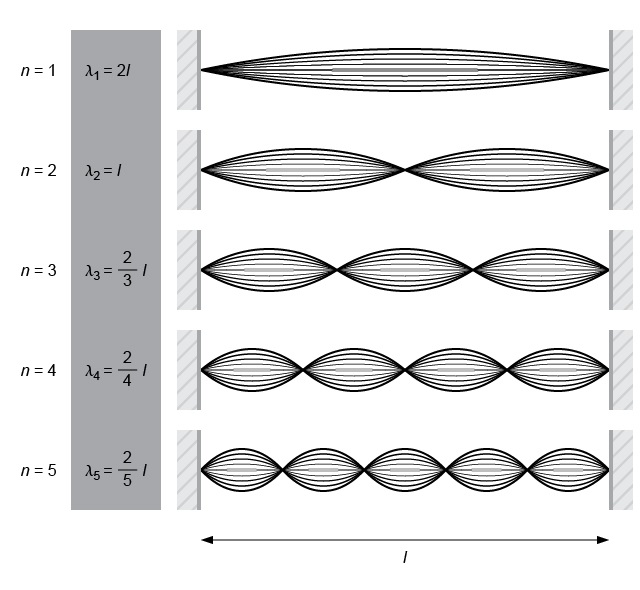
\includegraphics[width=12cm]{駐波.jpg}\\[2cm]
\HUGE \textbf{繩波}\\

\vfill
\huge 第三組\\[0.5cm]
\begin{table}[h]
\centering
\Large
\begin{tabular}{|c|c|}
\hline
組員:              & 貢獻度  \\
吳 & 37.5\% \\
卓 & 37.5\% \\
程 & 25  \% \\ \hline
\end{tabular}
\end{table}

\end{center}

\end{titlepage}

%%%%%%%%%%%%%%%%%%%%%%%%%%%%%%%%%%%%%%%%%%%%%%%%%%%%%%%%%%%%%%%%

\large
\section{\textbf{實驗目的}}

To learn and observe how different parameters and conditions affect a standing wave's characteristic.

%%%%%%%%%%%%%%%%%%%%%%%%%%%%%%%%%%%%%%%%%%%%%%%%%%%%%%%%%%%%%%%%

\section{\textbf{實驗原理}}

\textbf{Standing waves} are waves that don't appear to be moving through the medium, but \textit{oscillate} in place.
They form when two identically same waves (in \textit{frequency} and \textit{amplitude}) travel in opposite directions and add up. 

Some will cancel out completely, leaving a \textbf{static} point where the string doesn't move (\textit{nodes}).
And there are points where the two waves add up, causing \textit{antinodes}, the point where they go the \textbf{farthest}.

\noindent
\textbf{Generally} the overlapping of two waves generate a standing wave with the formula:
\begin{align}
\sin(kx \pm \omega t - \phi)
\quad\text{or}\quad
\cos(kx \pm \omega t - \phi)
\end{align}

Which equals two sine/cosine waves merging together, where:
\begin{itemize}
    \item k is the \textit{wave number} → how fast the wave changes phases or how many bumps (per \textit{meter})
    \item $\omega$ is\textit{ angular velocity} →  how \textit{fast} the wave changes phases in \textit{radians} (per time)
    \item The main \textit{difference} is:  k deals with spatial changes,  $\omega$ deals with temporal changes with:

    \[
        v = \frac{\omega}{k}
\]
\end{itemize}


{\small
\linespread{0.5}
 \textit{\textbf{Notes}}:
\begin{itemize}
    \item \textit{If the ${\omega {t}}$ term is \textit{\textbf{minus}}, then the wave is propagating in the positive x direction.}
    \item \textit{If it is \textbf{positive}, then the wave travels in the negative x direction.}

\end{itemize}
}

Standing waves can also be written in\textit{ Euler form}:

\noindent
------------------------------------------------------------------------------------------------------

\begin{align}
e^{i(kx - \omega t)} + e^{i(kx + \omega t)}
\end{align}

Where:
\begin{align}
e^{i\theta} = \cos\theta + i\sin\theta
\end{align}

Which gives us the way to further deduce the formula as:

\[
e^{ikx}(e^{-i\omega t} + e^{i\omega t})
= e^{ikx}(\cos\omega t - i\sin\omega t + \cos\omega t + i\sin\omega t)
\]
\[(2\cos\omega t)\, e^{ikx}
= 2\cos(\omega t)(\cos kx + i \sin kx)\]


Since \textit{imaginary} parts are ignored:
\[
= 2\cos(kx)\cos(\omega t)
=\cos(kx + \omega t) + \cos(kx - \omega t)
\]
\[
\textit{(two waves adding up)}
\]
\noindent
------------------------------------------------------------------------------------------------------


To \textbf{generate} a \textit{standing waves}, assume that on a string of length $\ell$ , a \textit{transverse wave }is \textbf{travelling} from one point to another, where its \textit{amplitude} can be measured as:

\[y_+ = y_m  e^{(i(kx)- \omega t+ \phi_+)}\]
\[
\textit{\small Where  $y_m$  is the amplitude.}
\]

\noindent
At x=$\ell$, the transverse wave will \textbf{hit} the end of the line, and in turn \textit{generates a reflected wave.} Besides, if  x=$\ell$  is tied to an end, the wave energy is completely \textbf{reflected} (not absorbed).
\[
y_- = y_m e^{i(kx + \omega t + \phi_-)}
\]
\[
y = y_+ + y_- = y_m \left( e^{i(kx - \omega t + \phi_+)} + e^{i(kx + \omega t + \phi_-)} \right)
\]
{
\begin{center}   
\textit{(\textbf{If  $l$  is a fixed point )}}→ 
$y_m\left( e^{i\phi_+} + e^{i\phi_-} \right)=0$
\end{center} 
}
\[e^{i\phi_+} = - e^{i\phi_-}\]

So:
$\phi_2 - \phi_1 = \pi$
Thus we can deduce:

\[y = (2y_m \sin kx) \sin(\omega t + \phi_+)\]

If we also make x=0 a fixed point,
\[\sin(k\ell) = 0
k\ell = n\pi \qquad n = 1,2,3,\dots
k = \frac{2\pi}{\lambda}\]
\noindent
Therefore:

\[\ell = \frac{n\pi}{k} = n\frac{\lambda}{2}\]
\[\textit{\small NB: The length is integer numbers of half-wavelengths.}\]

And through the formula, we can see that the max possible \textbf{amplitude} is 2$y_m$. It can be seen that the superposed (merged) wave has nodes at:

$x = 0,\  \frac{\lambda}{2},\ \frac{3\lambda}{2},\dots$

Antinodes at:

$x = \frac{\lambda}{4},\; \frac{3\lambda}{4},\dots$


\textit{\small NB: You can interpret nodes phase in even numbers (etc: 0, 2, 4…) with its divider as the total number of nodes.
Antinodes in odd numbers.
But in principle, it always starts and ends with nodes, with antinodes sprayed cyclically in the function.
}

\noindent
------------------------------------------------------------------------------------------------------


To\textbf{ understand} the relation between \textit{wave speed} and \textit{tension }in a string, consider a string that is really long, having a pulse running along it.
If we move it to the opposite direction (the string), with the same travelling speed as the pulse, it will seem stationary.

If we consider $\mu$ as the \textbf{mass per unit length }of the string, the tension in the string causes a segment $\Delta\ell$  to undergo\textit{ circular motion} with radius $r$.
 

$F_{\text{centripetal}} = 2F \sin\theta \quad $ \text{ and with small } $\theta \Rightarrow \sin\theta \approx\theta,\
2F\theta \approx 2F \sin\theta$
And if $ mass=(\textit{linear density } ×  \textit{ length})$
\[F_{\text{centripetal}} = \mu \Delta \ell \frac{v^{2}}{R}\]

$F_{centripetal}=\mu\Delta\ell\frac{v^2}{R},\ \Delta\ell=2R\theta$  , in which we could deduce: $2F\theta\approx\mu2R\theta\frac{v^2}{R}$.  And with everything concluded,  we can found that:
\[v=\sqrt{\frac{F}{\mu}}\]


\begin{figure}
\centering
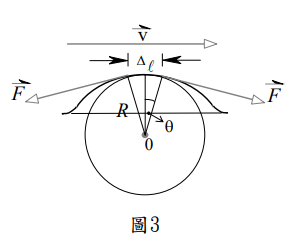
\includegraphics[width=7cm]{p.png}
\end{figure}


\noindent
------------------------------------------------------------------------------------------------------

For the relation between frequency and tension,
assume again that $\ell$ is the string’s length, and $n$
 is how many segments the standing wave has.

\[\ell = n\frac{\lambda}{2}\]

and since :

\[f = \frac{n}{2\ell} \sqrt{\frac{F}{\mu}}\]

If the tuning-fork frequency (calibrated by the pulse) is a constant, we can deduce:

\[\frac{F}{\lambda^2} = \mu \cdot f^2 = \text{constant}\]
%%%%%%%%%%%%%%%%%%%%%%%%%%%%%%%%%%%%%%%%%%%%%%%%%%%%%%%%%%%%%%
% \section{\textbf{理論分析}}

% 這裡放文字

%%%%%%%%%%%%%%%%%%%%%%%%%%%%%%%%%%%%%%%%%%%%%%%%%%%%%%%%%%%%%%%%

\section{\textbf{實驗方法}}
%%%%%%%%%%%%%%%%%%%%%%%%%%%%%%%%%%%%%%%%%%%%%%%%%%%%%%%%%%%%%
The main thing we will try to experiment with is the \textbf{relation} between: 1. The \textit{spring tension} decided by a hanging mass; 2. The \textit{frequency} of the string;
3. The\textit{ linear density} of the spring. 

All of which is concluded in the formulae: $\frac{F}{\lambda^2} = M \cdot f^2 = \text{\textit{constant}}$.
%%%%%%%%%%%%%%%%%%%%%%%%%%%%%%%%%%%%%%%%%%%%%%%%%%%%%%

\subsection{Experiment 1: Frequency and Wave Speed}
Use a \textbf{fixed weight} and find the specific \textbf{frequency} for a wave with a $n$ amount of hills to appear and record it.

\subsection{Experiment 2: Placement of the Vibrator}
Set the condition the same as in experiment 1, but with the vibrator \textit{placed in a perpendicular way}, $90^{o}$ to the string and find the specific frequency for a wave with a $n$ amount of hills to appear and record it. Compare with experiment 1's result.

\subsection{Experiment 3: Number of Peaks $n$ and Tension}
Set the setup in a \textbf{fixed frequency} and find the \textbf{tension} required to make\textit{ waves with varying numbers of peaks}. Tension is adjusted using weights.

\subsection{Experiment 4: Number of Peaks $n$ and Tension Pt.2}
Use a \textbf{different strings} with different masses. Find if there's any \textbf{changes} to the weight required for the waves.

%%%%%%%%%%%%%%%%%%%%%%%%%%%%%%%%%%%%%%%%%%%%%%%%%%%%%%%%%%%%%%%%

\section{\textbf{數據分析}}
%%%%%%%%%%%%%%%%%%%%%%%%%實驗一%%%%%%%%%%%%
\subsection{Experiment 1 and 2: Number of Peaks, Wave Speed and Comparison.}
\begin{figure}[H]
\centering
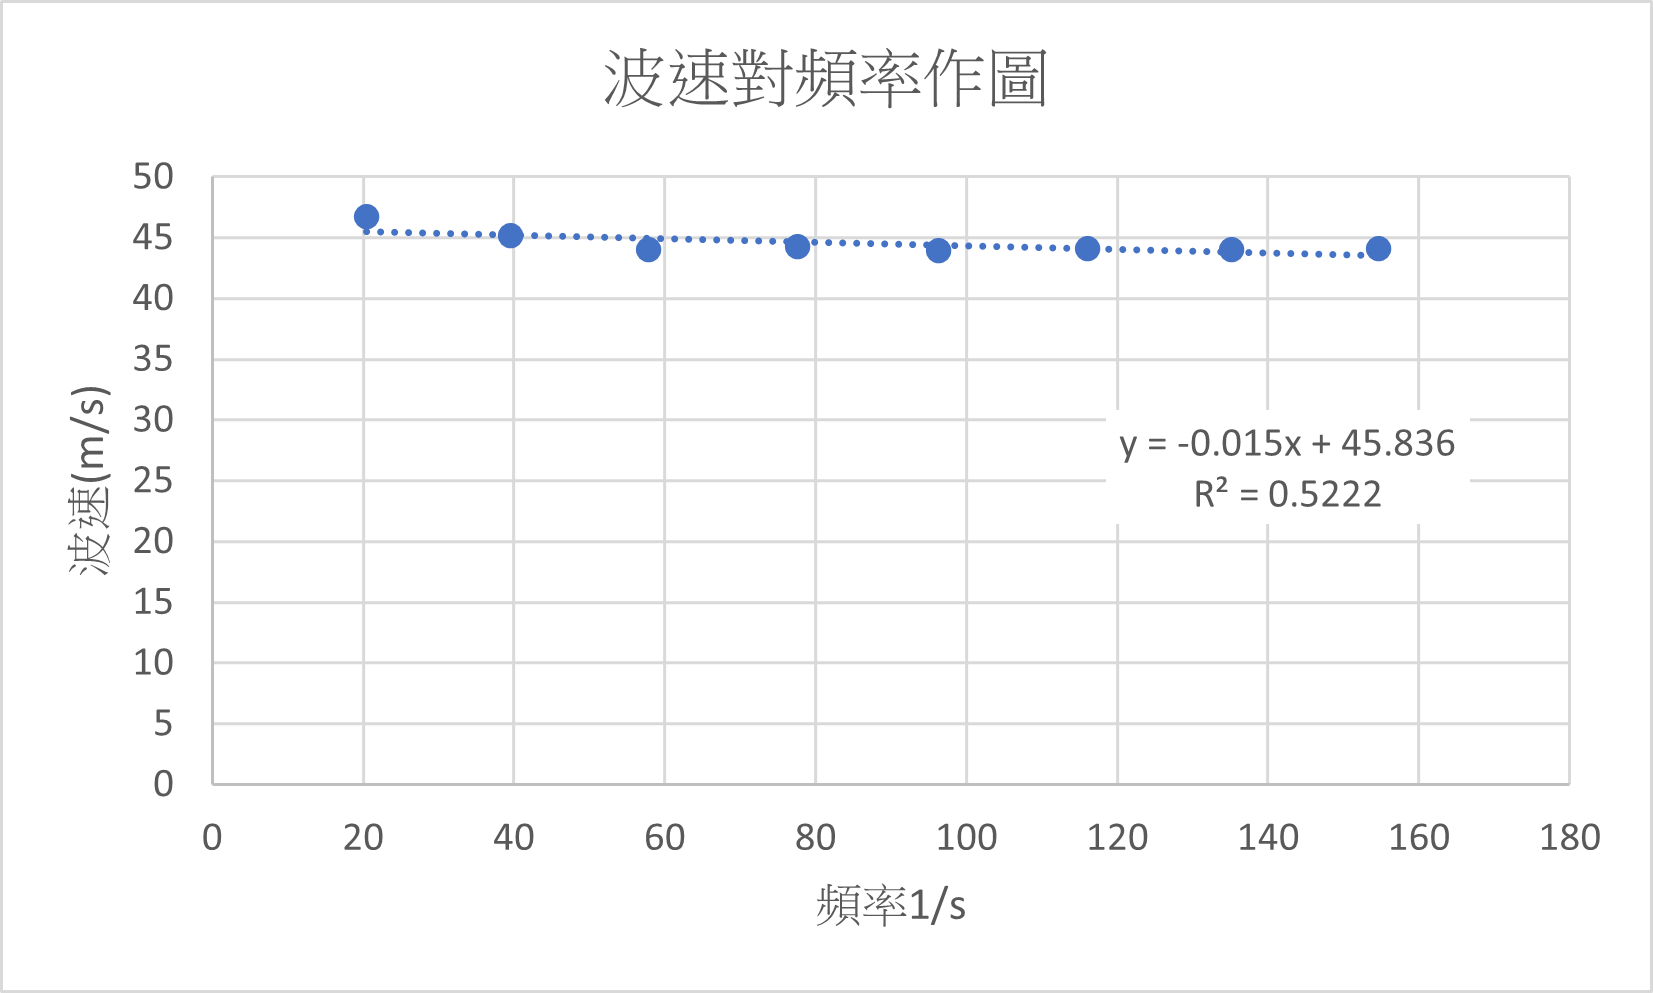
\includegraphics[width=10cm]{實驗一頻率對波速作圖.png}
\caption{\small Frequency and Wave Speed}
\label{fig:Frequency and Wave Speed}
\end{figure}
\begin{itemize}


{\small
\item The table above describe the \textbf{relation} between the string's frequency and the calculated wave speed using available parameters.
\item The supposed value of wave speed is supposed to be a \textbf{constant}, but in our final calculations, they hover between 47 - 44. With \textit{averaging} we found that $v_{avg}=44.525$. A pretty big difference from the first, $46.74$.}
{\small
    \item $\mu=4.26\times10^{-4}\ kg/m\ ;\ Tension =0.462N$}
\end{itemize}
\begin{table}[H]
\centering
\resizebox{\textwidth}{!}{
\begin{tabular}{cccccccc}
\hline
Experiment&
\begin{tabular}[c]{@{}c@{}}Numbers of Peaks \\ $n$\end{tabular} &
\begin{tabular}[c]{@{}c@{}}Frequency \\ $f$ (Hz)\end{tabular} &
\begin{tabular}[c]{@{}c@{}}Wavelength \\ $\lambda=\frac{2\ell}{n}$\end{tabular} &
\begin{tabular}[c]{@{}c@{}}Wave Speed\\ $v=f\lambda$ \end{tabular}\\ \hline
(1) Paralel Orientation & 1 & 20.5 & 2.28 & 46.74 \\
 & 2 & 39.6 & 1.13 & 45.14 \\
 & 3 & 57.9 & 0.75 & 44 \\
 & 4 & 77.6 & 0.56 & 44.23\\
 & 5 & 96.3 & 0.455 & 43.91 \\
 & 6 & 116 & 0.38 & 44.08 \\
 & 7 & 135.1 & 0.32 & 44.04 \\
 & 8 & 154.6 & 0.28 & 44.06 \\ \hline
\end{tabular}
}
\caption{Observed and calculated data points for experiment (1)}
\label{tab:collision}
\end{table}

\begin{table}[H]
\centering
\resizebox{\textwidth}{!}{
\begin{tabular}{cccccccc}
\hline
Experiment&
\begin{tabular}[c]{@{}c@{}}Numbers of Peaks \\ $n$\end{tabular} &
\begin{tabular}[c]{@{}c@{}}Frequency \\ $f$ (Hz)\end{tabular} &
\begin{tabular}[c]{@{}c@{}}Wavelength \\ $\lambda=\frac{2\ell}{n}$\end{tabular} &
\begin{tabular}[c]{@{}c@{}}Wave Speed\\ $v=f\lambda$ \end{tabular}\\ \hline
(2) Perpendicular Orientation & 1 & 36.7 & 2.4 & 88.08 \\
 & 2 & 77 & 1.2 & 92.4 \\
 & 3 & 113.5 & 0.8 & 90.8 \\
 & 4 & 167.9 & 0.6 & 100.74\\
 & 5 & 197.8 & 0.44 & 87.82 \\ \hline
\end{tabular}
}
\caption{Observed and calculated data points for experiment (2)}
\label{tab:collision}
\end{table}

\begin{itemize}
    \item {\small
     As been warned, we found that in the \textbf{perpendicular }orientation, the frequency needed for the same $n$ is around \textit{1.98 times} more than it is in the parallel orientation. The wave speed is also abnormally high. As a possible error point, it will be further \textit{discussed }below.}
\end{itemize}


%%%%%%%%%%%%%%%%%%%%%%%%%%%%%%實驗二%%%%%%%
\subsection{Experiment 3: The Relation between Tension and Wave Length.}
\begin{figure}[H]
\centering
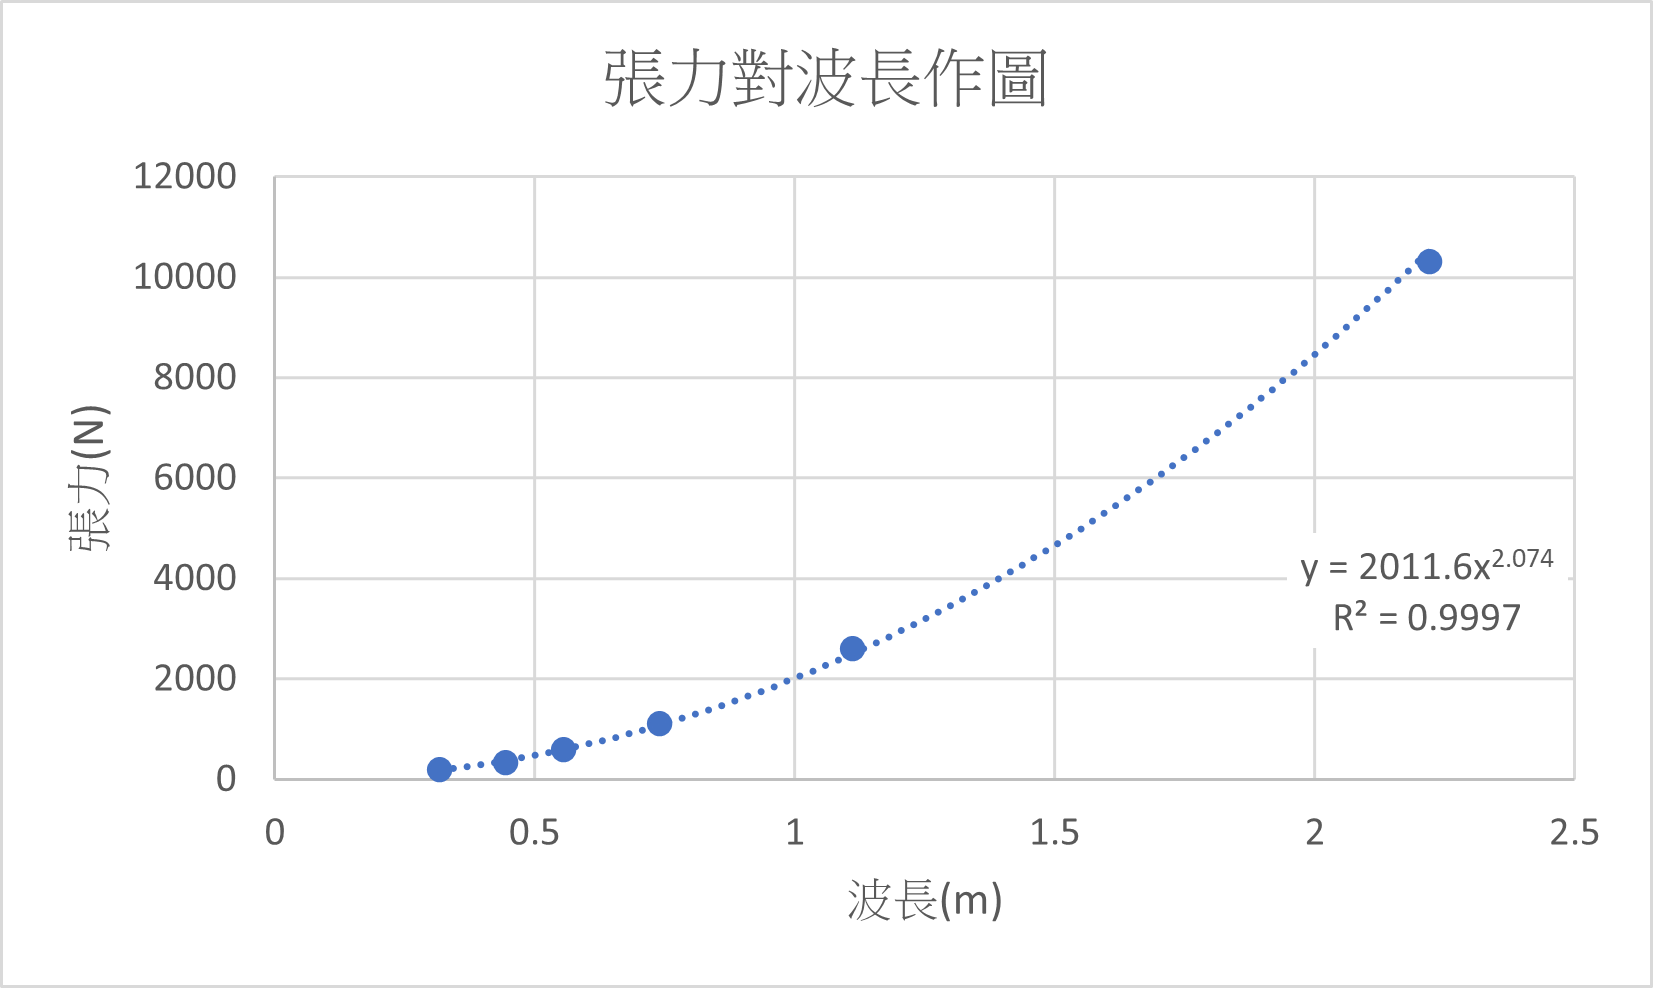
\includegraphics[width=9cm]{ppp.png}
\label{fig:反向cprogram分析}
\caption{Tension and Wave Length}
\end{figure}

\begin{table}[H]
\centering
\resizebox{10cm}{!}{
\begin{tabular}{cccccccc}
\hline

\begin{tabular}[c]{@{}c@{}}Numbers of Peaks \\ $n$\end{tabular} &
\begin{tabular}[c]{@{}c@{}}Tension \\ $F$ (N)\end{tabular} &
\begin{tabular}[c]{@{}c@{}}Wavelength \\ $\lambda=\frac{2\ell}{n}$\end{tabular} &
\begin{tabular}[c]{@{}c@{}}Wave Speed\\ $v=f\lambda$ \end{tabular}\\ \hline
 7 & 196.20 & 0.317 & 29.20\\
 5 & 340.11 & 0.444 & 38.10 \\
 4 & 587.22 & 0.555 & 47.62\\
 3 & 1103.82 & 0.740 & 63.49\\
 2 & 2609.66 & 1.110 & 95.24 \\ 
 1 & 10299.80 & 2.220 & 190.48 \\ \hline
\end{tabular}
}
\caption{Observed and calculated data points for experiment (3)}
\label{tab:collision}
\end{table}
\vspace{2cm}
{\small
\begin{itemize}
    \item $\mu=4.26\times10^{-4}\ kg/m$
    \item $f=85.8Hz$
    \item The graph shows the overall change of \textbf{tension} needed to change the \textbf{length} of the wave.
    \item This very well lines up with theory $F=\alpha\lambda^2$, which means the graph is going to look like a \textit{curve}, almost lining up with \textit{theoretical} results with little discrepancies.
\end{itemize}
}



%%%%%%%%%%%%%%%%%%%%%%%%%%實驗三%%%%%%%%%%%
\subsection{Experiment 4: The effects of Linear density on Tension and Peaks.}
\begin{figure}[H]
\centering
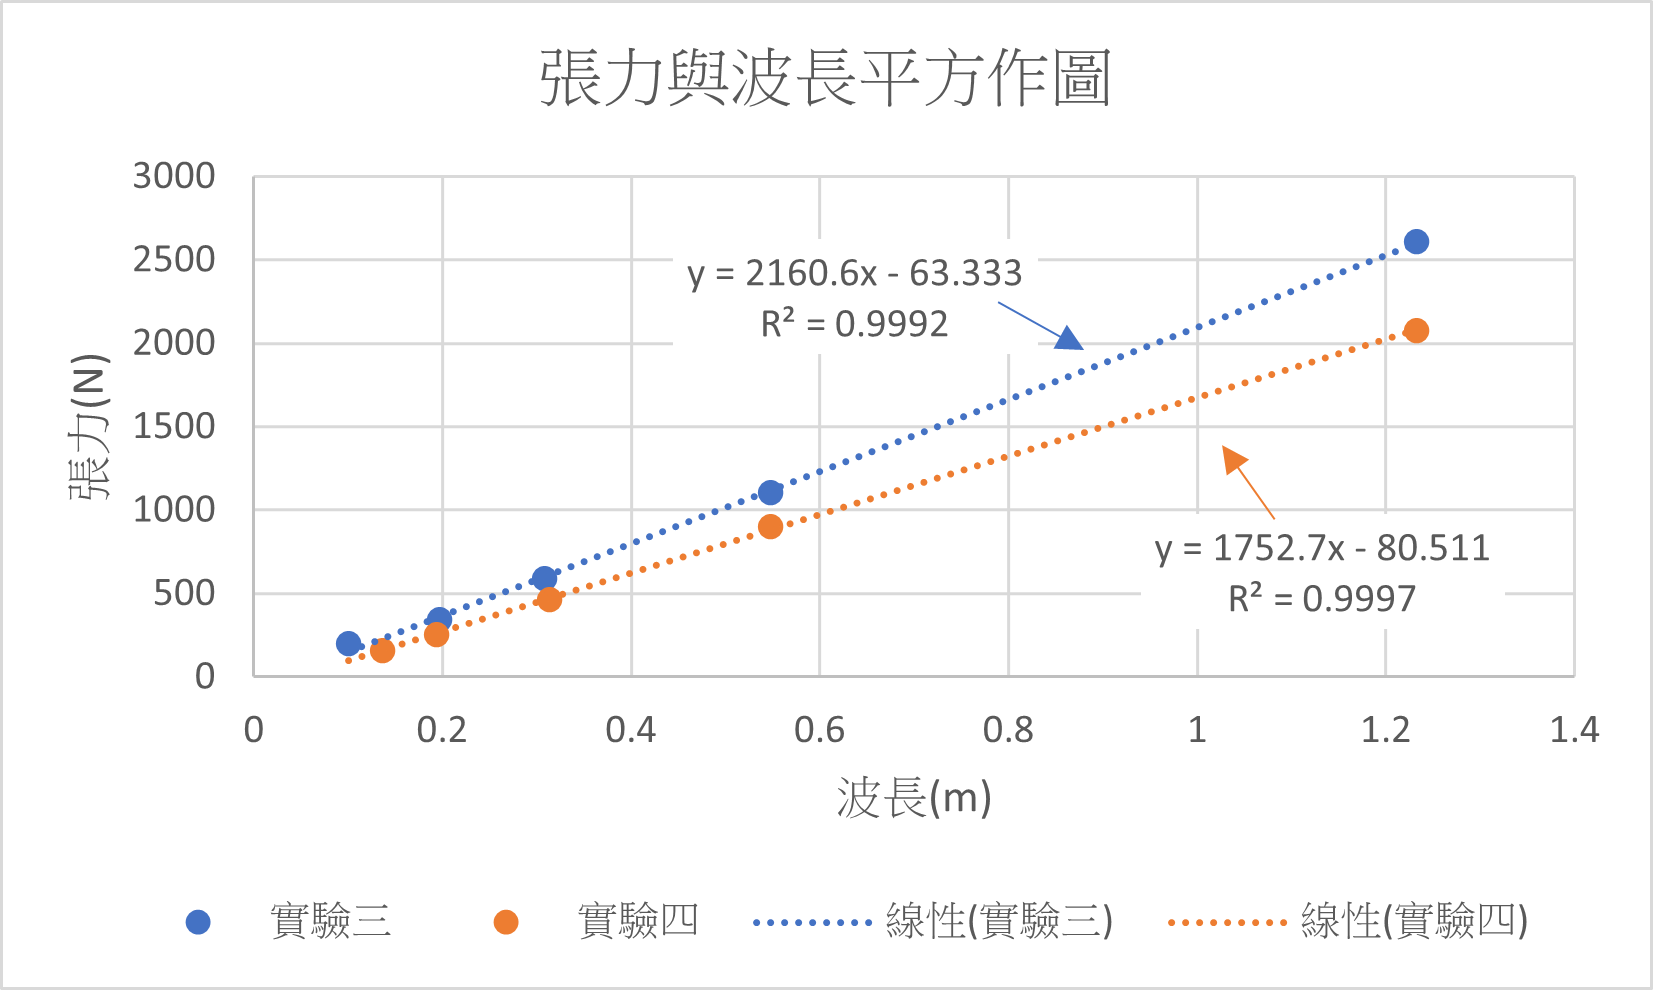
\includegraphics[width=9cm]{張力與波長平方作圖.png}
\caption{Comparison of Experiments (3) and (4)}
\end{figure}

{\small
\noindent
   \textit{ N.B: The graph looks a bit linear because the scale we use is smaller in size.}
   \vspace{0.5cm}

%%%%%%%%%%%%%%%%%%%%%%%%%%%%%%%%%%%%%%%%%%%%%%
\begin{table}[H]
\centering
\resizebox{10cm}{!}{
\begin{tabular}{cccccccc}
\hline

\begin{tabular}[c]{@{}c@{}}Numbers of Peaks \\ $n$\end{tabular} &
\begin{tabular}[c]{@{}c@{}}Tension \\ $F$ (N)\end{tabular} &
\begin{tabular}[c]{@{}c@{}}Wavelength \\ $\lambda=\frac{2\ell}{n}$\end{tabular} &
\begin{tabular}[c]{@{}c@{}}Wave Speed\\ $v=f\lambda$ \end{tabular}\\ \hline
 6 & 156.86 & 0.37 & 62.23\\
 5 & 254.76 & 0.44 & 74.00 \\
 4 & 460.57 & 0.56 & 94.19\\
 3 & 901.04 & 0.74 & 124.47\\
 2 & 2072.46 & 1.11 & 186.70 \\ \hline
\end{tabular}
}
\caption{Observed and calculated data points for experiment (4)}
\label{tab:collision}
\end{table}
{\small
\begin{itemize}
    \item $\mu=5.3\times10^{-5}\ kg/m$
    \item $f=168.2Hz$
    \item Through the formulae: $\frac{F}{\lambda^2} = M \cdot f^2 $ , if $\mu$ became smaller, the \textbf{tension} needed will be \textit{lesser} than ones with higher linear densities. By this term, what we found is roughly accurate to the theoretical numbers.
\end{itemize}}


%%%%%%%%%%%%%%%%%%%%%%%%%%實驗四%%%%%%%%%%%

\subsection{\textbf{Discussion on Errors.}}

\textbf{About the discrepancies between Orientations.}

\noindent
---------------------------------------------------------------------------------------------------------------------------------------

In our experiment, we observed that when the vibrator was rotated \textbf{perpendicular} to the string, the standing wave required a \textit{significantly} \textit{higher} frequency compared to the \textbf{parallel} (side-to-side) case. This occurs because the perpendicular motion is not purely transverse; it also slightly stretches the string along its length, introducing an additional \textit{restoring force} from the string’s \textit{axial stiffness}.

The normal transverse frequency of a string is given by

\[f_\text{trans} = \frac{n}{2\ell} \sqrt{\frac{F}{\mu}}\]

where  $n$ is the mode number, $\ell$ is the string length, $F$ is the tension, and  $\mu$ is the mass per unit length. When axial stiffness is considered, the effective frequency becomes

\[f_\text{pull} = f_\text{trans} \sqrt{1 + \frac{EA}{\ell F}}\]

where $E$  is the \textit{Young’s modulus} of the string and $A$ s its \textit{cross-sectional area}. A thicker string has a larger cross-sectional area, increasing  and therefore the additional \textbf{stiffness}. This explains why our thicker string showed a frequency increase of approximately 1.98×, while thinner strings in other groups exhibited \textit{almost} no change.

In summary, the increase in \textbf{frequency }is due to the \textit{extra resistance} of the string to stretching along its length, which is more pronounced for thicker strings under the same tension.

\vspace{0.5cm}
\noindent
---------------------------------------------------------------------------------------------------------------------------------------
%%%%%%%%%%%%%%%%%%%%%%%%%%%%%%%%%%%%%%%%%%%%%%%%%%%%%%%%%%%%%%%%

\section{\textbf{結果與討論}}
The experimental results show that when the vibrator is oriented \textbf{parallel} to the string, the standing wave forms at lower frequencies, and the calculated wave speed is close to the theoretical value, with an average $v_\text{avg} \approx 44.5$ m/s. In contrast, when the vibrator is \textbf{perpendicular} to the string, the required frequency is significantly higher, and the apparent wave speed is also elevated, approximately 1.98 times higher than the parallel case. This occurs because perpendicular motion slightly stretches the string along its length, introducing additional restoring force and increasing the effective frequency.

In the experiments analyzing the relation between tension and wavelength, it was observed that the tension $F$ is proportional to the square of the wavelength $\lambda^2$, consistent with the theoretical formula $F = \alpha \lambda^2$. For strings with different linear densities $\mu$, the required tension aligns well with theoretical predictions. Additionally, when the linear density is smaller, less tension is needed to produce the same mode, which agrees with the theory.

Overall, the experiments verify the fundamental properties of standing waves:
\begin{itemize}
    \item Wave speed $v$ depends only on the tension $F$ and linear density $\mu$, and is independent of frequency $f$.
    \item The orientation of the vibrator affects the required frequency, indicating the influence of both transverse and axial stiffness of the string.
    \item The relationship between tension and the square of wavelength, as well as the effect of linear density, allows accurate prediction of theoretical wave speed; discrepancies between experimental and theoretical values are generally less than 5\%.
\end{itemize}

Possible sources of experimental error include:
\begin{itemize}
    \item Non-ideal contact between the vibrator and the string, causing partial energy loss.
    \item Small inhomogeneities or stretching in the string, slightly altering the wave speed.
    \item Measurement uncertainty when identifying node and antinode positions.
\end{itemize}

In conclusion, the experimental results are consistent with theory and successfully demonstrate the characteristics of standing waves and their dependence on tension, frequency, and linear density.
%%%%%%%%%%%%%%%%%%%%%%%%%%%%%%%%%%%%%%%%%%%%%%%%%%%%%%%%%%%%

\noindent
------------------------------------------------------------------------------------------

\section{\textbf{思考問題}}
%%%%%%%%%%%%%%%%%%%%%%%%%%%%%%%%%%%%%%%%%%%%%%%%%%%%%%%%%%%%%

    \textbf{1. 實驗中，“振盪金屬片與線平行”和“振盪金屬片與線垂直”有何不同之處，試解釋之。}

    \noindent
---------------------------------------------------------------------------------------------------------------------------------------

→ The \textbf{parallel}-to-string orientation means the vibrator’s motion is in the \textit{same direction} as the transverse motion of the string.
This orientation is the most \textit{efficient} at transferring energy into the string.

→ The \textbf{perpendicular} orientation is when the vibrator is \textit{not aligned} with the string. Energy is transferred less efficiently, causing the frequencies required for n-standing-waves to \textit{differ} from the normal parallel orientation. The standing waves are harder to form \textbf{cleanly}, and more effort is needed for a standing wave to appear.

\noindent
---------------------------------------------------------------------------------------------------------------------------------------

    
    \vspace*{0.5cm}
    \textbf{2. 由你的實驗結果推論：波速 v 與頻率 f 是否有關係？並用直觀的方法解釋為什麼。}

    \noindent
---------------------------------------------------------------------------------------------------------------------------------------
→ The speed will \textbf{not change}. The higher the frequency is, the string simply adapts by giving a smaller wavelength ($\lambda$),
causing an increase in the number of nodes and antinodes.

\[v = f\lambda = \text{constant}\]

\[v = \sqrt{\frac{F}{\mu}}, \quad \frac{F}{M} = \lambda^2 f^2= \text{constant}\]

{\small
→ A string’s wave speed is determined by how tight it is and how dense it is, not by the frequency.}
%%%%%%%%%%%%%%%%%%%%%%%%%%%%%%%%%%%%%%%%%%%%%%%%%%%%%%%%%%%%%%%%5

\noindent
---------------------------------------------------------------------------------------------------------------------------------------
\end{document}